
\subsection{Adding Two Positive Integers}


\subsection{Adding a Positive and a Negative Integer}


\subsection{Adding Two Negative Integers}
Lastly, let's add $(-5) + (-3)$:
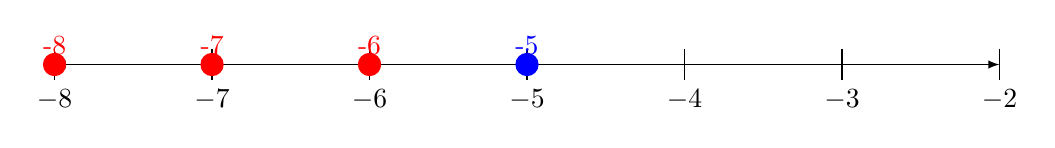
\begin{tikzpicture}[scale=2]
    % Numeric line
    \draw[latex-latex] (-8,0) -- (-2,0);
    \foreach \x in {-8,-7,-6,-5,-4,-3,-2}
    \draw (\x,0.1) -- (\x,-0.1);
    \foreach \x/\label in {-8/-8,-7/-7,-6/-6,-5/-5,-4/-4,-3/-3,-2/-2}
    \node[below] at (\x,-0.1) {$\label$};

    % Starting point
    \filldraw[blue] (-5,0) circle (2pt) node[above] {-5};

    % Moving left
    \filldraw[red] (-5-1,0) circle (2pt) node[above] {-6};
    \filldraw[red] (-5-2,0) circle (2pt) node[above] {-7};
    \filldraw[red] (-5-3,0) circle (2pt) node[above] {-8};
\end{tikzpicture}

So, $(-5) + (-3) = -8$.

\section{Subtracting Integers}
Subtracting integers can be thought of as adding the opposite (or additive inverse) of the number. Let's see some examples:

\subsection{Subtracting a Positive Integer}
Consider $7 - 3$:
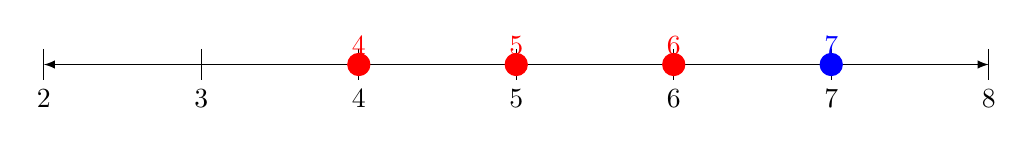
\begin{tikzpicture}[scale=2]
    % Numeric line
    \draw[latex-latex] (2,0) -- (8,0);
    \foreach \x in {2,3,4,5,6,7,8}
    \draw (\x,0.1) -- (\x,-0.1);
    \foreach \x/\label in {2/2,3/3,4/4,5/5,6/6,7/7,8/8}
    \node[below] at (\x,-0.1) {$\label$};

    % Starting point
    \filldraw[blue] (7,0) circle (2pt) node[above] {7};

    % Moving left
    \filldraw[red] (7-1,0) circle (2pt) node[above] {6};
    \filldraw[red] (7-2,0) circle (2pt) node[above] {5};
    \filldraw[red] (7-3,0) circle (2pt) node[above] {4};
\end{tikzpicture}

So, $7 - 3 = 4$.

\subsection{Subtracting a Negative Integer}
Now, let's subtract $5 - (-2)$:
\begin{tikzpicture}[scale=2]
    % Numeric line
    \draw[latex-latex] (-3,0) -- (6,0);
    \foreach \x in {-3,-2,-1,0,1,2,3,4,5,6}
    \draw (\x,0.1) -- (\x,-0.1);
    \foreach \x/\label in {-3/-3,-2/-2,-1/-1,0/0,1/1,2/2,3/3,4/4,5/5,6/6}
    \node[below] at (\x,-0.1) {$\label$};

    % Starting point
    \filldraw[blue] (5,0) circle (2pt) node[above] {5};

    % Moving right
    \filldraw[red] (5+1,0) circle (2pt) node[above] {6};
    \filldraw[red] (5+2,0) circle (2pt) node[above] {7};
    \filldraw[red] (5+3,0) circle (2pt) node[above] {8};
\end{tikzpicture}

So, $5 - (-2) = 8$.

\subsection{Subtracting Two Negative Integers}
Lastly, let's subtract $(-4) - (-7)$:
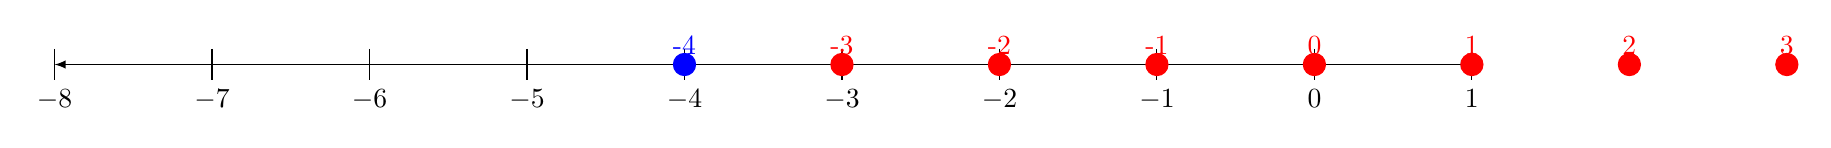
\begin{tikzpicture}[scale=2]
    % Numeric line
    \draw[latex-latex] (-8,0) -- (1,0);
    \foreach \x in {-8,-7,-6,-5,-4,-3,-2,-1,0,1}
    \draw (\x,0.1) -- (\x,-0.1);
    \foreach \x/\label in {-8/-8,-7/-7,-6/-6,-5/-5,-4/-4,-3/-3,-2/-2,-1/-1,0/0,1/1}
    \node[below] at (\x,-0.1) {$\label$};

    % Starting point
    \filldraw[blue] (-4,0) circle (2pt) node[above] {-4};

    % Moving right
    \filldraw[red] (-4+1,0) circle (2pt) node[above] {-3};
    \filldraw[red] (-4+2,0) circle (2pt) node[above] {-2};
    \filldraw[red] (-4+3,0) circle (2pt) node[above] {-1};
    \filldraw[red] (-4+4,0) circle (2pt) node[above] {0};
    \filldraw[red] (-4+5,0) circle (2pt) node[above] {1};
    \filldraw[red] (-4+6,0) circle (2pt) node[above] {2};
    \filldraw[red] (-4+7,0) circle (2pt) node[above] {3};
\end{tikzpicture}

So, $(-4) - (-7) = 3$.